\scanpage{5}
\mspage{3}
\deleted{\unsure{les $\pi_i$ de degré zéro}, et que} l'on \unsure{voudra|considère} que
\figure{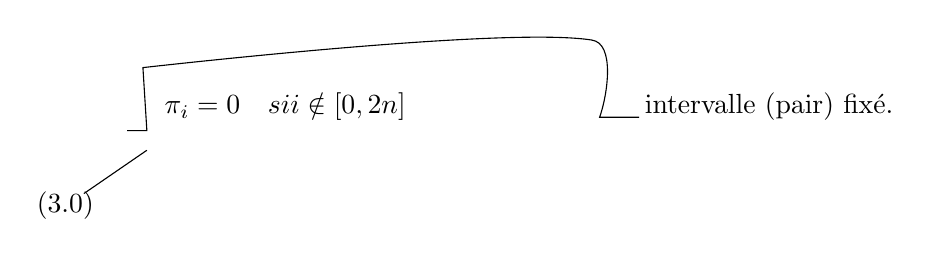
\begin{tikzpicture}[x=1cm,y=1cm]
\node[anchor=west] at (.8,.55) {$\pi_i=0\quad\text{si }i\notin[0,2n]$};
\node[anchor=west] at (6.9,.55) {intervalle \inserted{(pair)} fixé.};
\node[anchor=east] at (.15,-.7) {$(3.0)$};
\draw (.45,.25)--(.7,.25)--(.65,1.05) .. controls (2,1.2) and (5.4,1.55) .. (6.35,1.4) .. controls (6.65,1.36) and (6.55,.7) .. (6.45,.42)--(6.95,.42);
\draw (.7,0)--(-.1,-.55);
\end{tikzpicture}}
\deleted{\unsure{Supp}} On s'occupe ici de l'\uline{unicité}. \deleted{\unsure{Supposons, établie l'unicité}}

Notons d'abord que
\[
\mathcal E^0\ni u\quad\Longleftrightarrow\quad(u\pi_i=\pi_i u\quad\forall i)
\]
donc $\mathcal E^0$ est le commutant de la $k$-algèbre engendrée par les $\pi_i$. Donc les $\pi_i$ sont dans le centre $\unsure{Z|\mathfrak Z}(\mathcal E^0)$ de $\mathcal E^0$, et ce sont des projecteurs \inserted{mutuellement} orthogonaux de somme $1$ de cet anneau commutatif. Supposons déterminés déjà les $\pi_\alpha$ pour $\alpha\notin[i,2n-i]$, \inserted{$i<n$,} et déterminons $\pi_i$ et $\pi_{2n-i}$ [i.e. $\pi_\alpha$ pour $\alpha\notin[i+1,2n-i-1]$.]
\inserted{\figure{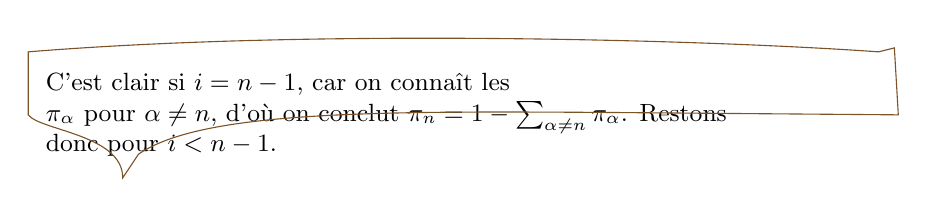
\begin{tikzpicture}[x=1cm,y=1cm]
\node[anchor=north west,align=left,font=\small] at (.2,.8) {C'est clair si $i=n-1$, car on connaît les\\$\pi_\alpha$ pour $\alpha\neq n$, d'où on conclut $\pi_n=1-\sum_{\alpha\neq n}\pi_\alpha$. \unsure{Restons}\\donc pour $i<n-1$.};
\draw[draw=brown!65!black] (.1,.95) .. controls (3.8,1.25) and (8.8,1.1) .. (10.9,.95) --(11.1,1.0)--(11.15,.15)--(7.5,.18) .. controls (4.5,.2) and (2.3,.2) .. (1.5,-.35) --(1.3,-.65) .. controls (1.3,-.1) and (.25,-.05) .. (.1,.15)--cycle;
\end{tikzpicture}}}
On connaît donc
\[
\varphi_i=\deleted{\unsure{1-\sum\pi_\alpha}}\left(1-\sum_{\alpha<i}\pi_{\unsure{i|\alpha}}\right)=\sum_{\alpha\geq i}\pi_\alpha,
\quad\text{et}\quad
\psi_{2n-i}=\left(1-\sum_{\alpha>2n-i}\pi_{\unsure{i|\alpha}}\right)=\sum_{\alpha\leq 2n-i}\pi_\alpha
\]
donc aussi la composante
\[
\unsure{ou}\quad\psi_{2n-i}\deleted{\unsure{\varphi}}\mathcal E^{2n-2i}\varphi_i
=\sum_\alpha\psi_{2n-i}\pi_{\alpha+(2n-2i)}\mathcal E\pi_\alpha\varphi_i\unsure{)}
\]
Or
\[
\pi_\alpha\varphi_i=\begin{cases}0&\text{si }\alpha<i\\\pi_\alpha&\text{si }\alpha\geq i\end{cases}
\quad\text{et}\quad
\psi_{2n-i}\pi_{\alpha+(2n-2i)}=
\begin{cases}
0&\text{si }\inserted{\alpha+(2n-2i)>2n-i}\quad\text{i.e. }\alpha>i\\
\pi_{\alpha+(2n-2i)}&\text{si }\inserted{\alpha\leq i}
\end{cases}
\]
donc le terme d'indice $\alpha$ de la somme $\sum$ est nul sauf si $\alpha=i$, auquel cas il est égal à
\[
\pi_{\unsure{i|\alpha}+(2n-2i)}\mathcal E\pi_i=\pi_{2n-i}\mathcal E\pi_i=\mathcal E_{2n-i,i}.
\]
Donc la connaissance des $\pi_\alpha$ pour $\alpha\notin[i,2n-i]$ implique la connaissance de $\mathcal E_{\deleted{\unsure{i,2n-i}}\inserted{2n-i,i}}$ \deleted{\unsure{Consid}}

La condition qui va impliquer l'unicité \deleted{\unsure{de}} de $\unsure{u_i|\pi_i}$,
\mspage{4}
